\chapter{Safety}
\label{sec-safety}
\newcounter{tcheckcnt}
\newcommand{\tcheck}[1]{\refstepcounter{tcheckcnt}T-\arabic{tcheckcnt}\label{#1}}
\newcounter{rcheckcnt}
\newcommand{\rcheck}[1]{\refstepcounter{rcheckcnt}R-\arabic{rcheckcnt}\label{#1}}

\makeatletter
\renewcommand\p@tcheckcnt{T-\arabic{tcheckcnt}\expandafter\@gobble}
\renewcommand\p@rcheckcnt{R-\arabic{rcheckcnt}\expandafter\@gobble}
\makeatother

\begin{table*}
\centering
\caption{List of safety checks}
\label{tbl-safety-checks}
\begin{tabular}{lp{0.9\linewidth}}
\toprule
 & Translation-time checks \\

\tcheck{chk-method-header-is-sane}
	& For each method header, the number of own local variable slots <= the number of total variable slots, the number of (int/ref) arguments <= the number of (int/ref) variables, static methods are not abstract. \\

\tcheck{chk-return-or-goto-at-end-of-method}
	& The last instruction of each method is a \mycode{RETURN} or \mycode{GOTO}. \\

\tcheck{chk-brtarget-exists}
	& Branch instructions branch to an index < the number of \mycode{BRTARGET}s announced in the method header. \\

\tcheck{chk-all-brtargets-found}
	& At the end of each method, we have seen the exact number of \mycode{BRTARGET} instructions announced in the method header. \\

\tcheck{chk-invokelight-target-found}
	& The target for an \mycode{INVOKELIGHT} call is already translated, so the target address is known. \\

\tcheck{chk-invokestatic-target-header-found}
	& The target method header for an \mycode{INVOKESTATIC}/\mycode{INVOKESPECIAL} exists. \\

\tcheck{chk-stack-is-empty-after-return}
	& After popping the return value, the stack is empty. \\

\tcheck{chk-sufficient-locals-at-invokelight}
	& For each \mycode{INVOKELIGHT}, the total number of slots - the number of own variable slots for the caller >= the total variable slots for the callee. \\

\tcheck{chk-sufficient-stack-space-at-invokelight}
	& At the point of an \mycode{INVOKELIGHT} instruction, the max stack of the caller >= the current stack depth - the number of arguments to the callee + the max stack of the callee. \\

\tcheck{chk-stack-is-empty-at-branches}
	& The stack is empty at branches and branch targets. \\

\tcheck{chk-no-operandstack-underflow}
	& Before each instruction, the stack depth >= the number of elements to be consumed by the instruction. \\

\tcheck{chk-no-operandstack-overflow}
	& After each instruction, the stack depth <= the max stack depth announced in the header. \\

\tcheck{chk-local-variable-slot-exists}
	& The index of the local variable < the number of own variable slots for the current method. \\

\tcheck{chk-static-variable-infusion-exists}
	& The target infusion of a static variable exists. \\

\tcheck{chk-static-variable-slot-exists}
	& The index of the static variable < the number of static variable slots for the target infusion. \\

\midrule
& Run-time checks \\

\rcheck{chk-invokevirtual-target-found}
	& The target implementation for an \mycode{INVOKEVIRTUAL}/\mycode{INVOKEINTERFACE} is found. \\

\rcheck{chk-no-nativestack-overflow}
	& Whenever a new stack frame is allocated the frame+max stack depth+some safety margin > the end of the heap. \\

\rcheck{chk-invokevirtual-stack-effects-match}
	& The target implementation for an \mycode{INVOKEVIRTUAL}/\mycode{INVOKEINTERFACE} matches the stack effects used to verify the caller's stack at translation time. \\

\rcheck{chk-memory-access-within-heap}
	& The target address of an array element or object field is within the heap. \\

\bottomrule
\end{tabular}
\end{table*}

The second goal of this dissertation is to develop a VM that offers a 'safe' execution environment, and to compare the cost of doing so using a VM to existing native code approaches.

A safe execution environment is one that guarantees an application cannot harm the system it is running on or other applications running on the same system. Specifically, an application cannot:
\begin{enumerate}
    \item Execute code it does not have permission for,
    \item Write to memory outside the areas assigned to it, or
    \item Retain control of the CPU indefinitely.
\end{enumerate}

Given the first two, the last guarantee is easy to implement: the VM can use interrupts or set a timer to trap back to the VM and regain control when needed. As long as the other guarantees hold, the application will not be able to disable these without the VM's permission.

To guard against programming errors as well as malicious attacks, we focus on the second type of approaches shown in Figure \ref{fig-safe-compilation-process}. CapeVM does not rely on a trusted host to guarantee safety, but can do so independent of the code it receives.

As discussed in Chapter 3, most generic sensor nodes VMs do not consider safety, with the exception of SensorScheme \cite{Evers:2010ur}, but a number of native code systems have been developed. This is unfortunate because using a VM has some distinct advantages compared to native code systems that guarantee safety.

Both the machine model and the instruction set of the virtual machine are more structured than a real CPU. This restricts what a bytecode instruction can do, which in turn allows the VM to verify safety for many instructions at translation time.

As an example, memory on the physical CPU is a flat address space, and the ATmega's store instructions can write to \emph{any} address in memory, which means any write could potentially corrupt memory. In the VM, memory for local variables, static variables, and for objects and arrays are separated, and the VM has separate instructions to target each of them as an offset within their respective regions. Similarly, native code can branch to any address within flash memory, while the VM's branches target the id of a branch target within the current method.

In CapeVM, the programme eventually also runs as native code on the physical CPU, but the VM is in complete control of how this code is generated and the context in which it runs. As shown in the next sections, this make it easy to determine at translation time that stores to local and static variables will write to space reserved for a local or static variable, and that branches will branch to a legal instruction within the method.

Table \ref{tbl-safety-checks} contains the list of checks done by CapeVM to guarantee safety. To show these are sufficient to satisfy the high level guarantees listed before, we first express them as concrete constraints specific to CapeVM:

\begin{itemize}
    \item \emph{Control flow safety}: after starting the application, the VM is always executing either
        \begin{itemize}
            \item a translated bytecode instruction in the current method \emph{from the start}, or
            \item code in the VM itself, as a result of either a call to a VM function from a translated bytecode instruction, or returning from a method.
        \end{itemize}
    \item \emph{Memory safety}: any write to memory done by the application is to a legal location: either
        \begin{itemize}
            \item memory reserved for the operand stack, or
            \item a valid local or static variable slot, or
            \item the area of the heap assigned to the application.
        \end{itemize}
\end{itemize}

The control flow guarantees make sure code cannot jump to a point half-way a generated instruction to skip run-time checks, or to anywhere in the VM except through the proper entry points defined by the VM. As in normal Java, the bytecode instructions in CapeVM can only modify state within the virtual machine. There are no special instructions to access sensors and actuators as in, for example, Maté. Thus, access to external resources is assumed to happen through calls to natively implemented library functions, which returns control to VM and allows it to check whether the application has permission to do so.

Clearly, the VM will be in a legal state when a programme starts: the VM will jump to the begining of the first instruction and no writes will have occured yet. We will show the checks in Table \ref{tbl-safety-checks} are sufficient to ensure these two constraints, by examining how each bytecode instruction can affect control flow and write to memory, and list the checks necessary to ensure the VM is still in a legal state after executing each instruction. Both guarantees depend on each other: memory safety is assumed when discussing control flow safety and vice versa.

Each method in CapeVM has a small \emph{method header} defining properties such as the maximum stack size, number of local variables, return type, etc. The VM uses this header to create the stack frame, and to determine the effects of a call to a method on the caller's operand stack. Therefore, many of the checks are to ensure the implementation of the method follows the contract established in the method header. When the node receives new code, it first receives the headers for all methods, followed by their implementations, so the contracts for all methods are known when the bytecode is translated.

The first check is a basic sanity check on the data in the method headers (\ref{chk-method-header-is-sane}). Since each parameter becomes a local variable, the number of local variable slots must be at least as high as the number of parameters, and the total number of slots must be at least as high as the method's own local variable slots, while the rest may be used for lightweight methods. Finally, a method cannot be marked static and abstract at the same time.

\section{Control flow safety}
We show control flow safety is guaranteed by our checks by considering all bytecode instructions, and showing they either flow into the start of a legal next instruction, or return control back to the VM. Regarding their effect on control flow, the bytecode instructions can be grouped into four categories, shown in Table \ref{tbl-control-flow-instructions}.

The state is correct at the start of the programme, since the VM will start it by jumping to the beginning of the first instruction in the main method. We will show the state will be correct after each following instruction by looking at these four categories.

\begin{table}
\caption{Instructions affecting control flow}
\label{tbl-control-flow-instructions}
    \begin{tabular}{ll} % NO SIMULATION DATA
    \toprule
    Type              & Effect on control flow \\
    \midrule
    \midrule
    Branches          & Jump to a location within the method \\
    \mycode{INVOKE}   & Call a method, either through the VM or directly \\
    \mycode{RETURN}   & Return to the address at the top of the stack \\
    Others            & Fall through to the next bytecode instruction \\
    \bottomrule
    \end{tabular}
\end{table}

\subsection{Simple instructions}
Starting with the last category: most instructions such as math operations, loads and stores, are translated to a sequence of native instructions that will be executed top to bottom. In some cases this may call to a VM or \mycode{libc} function to perform some complex operation, but these calls return to the current instruction once the operation is complete.

For this category, the generated code will naturally flow into the start of the next generated instruction. This is means the control flow constraint would be broken if there \emph{is no} next instruction, which produces the second translation-time check, \ref{chk-return-or-goto-at-end-of-method}: the last instruction in a method must be a \mycode{RETURN} or \mycode{GOTO} to prevent control from flowing out of the method body.

\subsection{Branch instructions}
In CapeVM bytecode, branches do not target an offset as in normal JVM bytecode, but the id of a branch target. These targets are marked with \mycode{BRTARGET} instructions, which do not emit any code, but cause the AOT compiler to collect the address in a temporary table during translation. Once the whole method is translated, this temporary table is used to patch the correct target address into the branch instructions.

Each method announces the number of branch targets that will be used in the method header. Non-taken branches flow into the next instruction because \ref{chk-return-or-goto-at-end-of-method} guarantees they are not the last instruction in a method. To ensure a taken branch will branch to the start of a correct instruction within the method, two checks are needed: the target ID of each branch must be lower than number of branch targets announced in the method header (\ref{chk-brtarget-exists}), and at the end of the method the number of \mycode{BRTARGET} instructions encountered must be equal to the number announced in the header (\ref{chk-all-brtargets-found}). The first guarantees each branch refers to an entry within the temporary table, while the second guarantees all entries are filled with a valid address.

\subsection{Method invocation instructions}
There are three kinds of method invocations.

For lightweight method calls, the implementation of the target method is required to come before any method invoking it, to ensure the address of the target is known at translation time and the VM can directly generate a \mycode{CALL} to the method. Ensuring this calls to a correct address is therefore trivial: for \mycode{INVOKELIGHT} instructions, the implementation of the target method must already have been generated (\ref{chk-invokelight-target-found}).

For static calls (\mycode{INVOKESTATIC} and \mycode{INVOKESPECIAL}) the target method is known at translation time, but it may not have been translated yet if the implementation follows later in the infusion. For these instructions, a \mycode{CALL} to the VM's \mycode{callMethod} function is generated, passing the id of the target method as a parameter. At run time this id will be used as an index in the method table to find its implementation. Because the VM receives all the method headers before translating their implementations, it can check at translation time that the method id is known (\ref{chk-invokestatic-target-header-found}). Since the VM will not start an application before all methods are translated, this guarantees that \mycode{callMethod} will find the target at run time.

Finally, for \mycode{INVOKEVIRTUAL} and \mycode{INVOKEINTERFACE}, the target is not known at translation time, since this depends on the object the method is invoked on. Darjeeling does not use dispatch tables to call virtual methods. Instead, each infusion contains a flattened list of methods that are scanned to find the right implementation for the current object. Therefore a run-time check is needed to verify the method can be found (\ref{chk-invokevirtual-target-found}), but since this is necessary to make the call, this check does not add any extra overhead.

Again, once the call returns, check \ref{chk-return-or-goto-at-end-of-method} ensures control will flow into a valid next instruction.

\subsection{Return instructions}
\label{sec-control-flow-safety-return-instructions}
Finally, return instructions pop the return value from the stack, and then emit a native \mycode{RET} instruction to exit the method and return control, either directly to the AOT compiled code of the caller for lightweight method calls, or to the VM's \mycode{callMethod} function for normal methods.

The \mycode{RET} instruction takes the return address from the native stack, which is also used to store the VM's integer operand stack. This means the integer operand stack needs to be empty at return instructions (\ref{chk-stack-is-empty-after-return}) to ensure the correct address will be at the top of the native stack. Memory safety then guarantees the application could not have corrupted it. Without this check, malicious code could leave an integer on the stack and use the return instruction to jump to an arbitrary location.

A second way the return address could be corrupted is if the native stack overflows into the VM's heap. In CapeVM the heap is a fixed sized block that sits above other global variables, and below the native stack that grows down towards it. If the native stack grows into the area reserved for the heap, a return address may be corrupted by an otherwise valid heap write.

To prevent this, a run-time check is added to non-lightweight invokes, that checks the stack frame for the called method, plus its maximum integer stack size, does not grow into the heap (\ref{chk-no-nativestack-overflow}). Lightweight calls do not add to the stack, since space for their local variables, stack, and return address was already allocated in the caller's frame.

While running, a method may make calls to the VM or \mycode{libc} functions, causing the native stack to grow further. Since the maximum stack growth for such calls is fixed, a certain safety margin is added between the stack and heap. A similar gap of 128 bytes between the stack and kernel heap is reserved by \emph{t-kernel} \cite{Gu:2005un}, although it is not clear from the paper whether this is for the same reason.




\section{Memory safety}

\begin{figure}
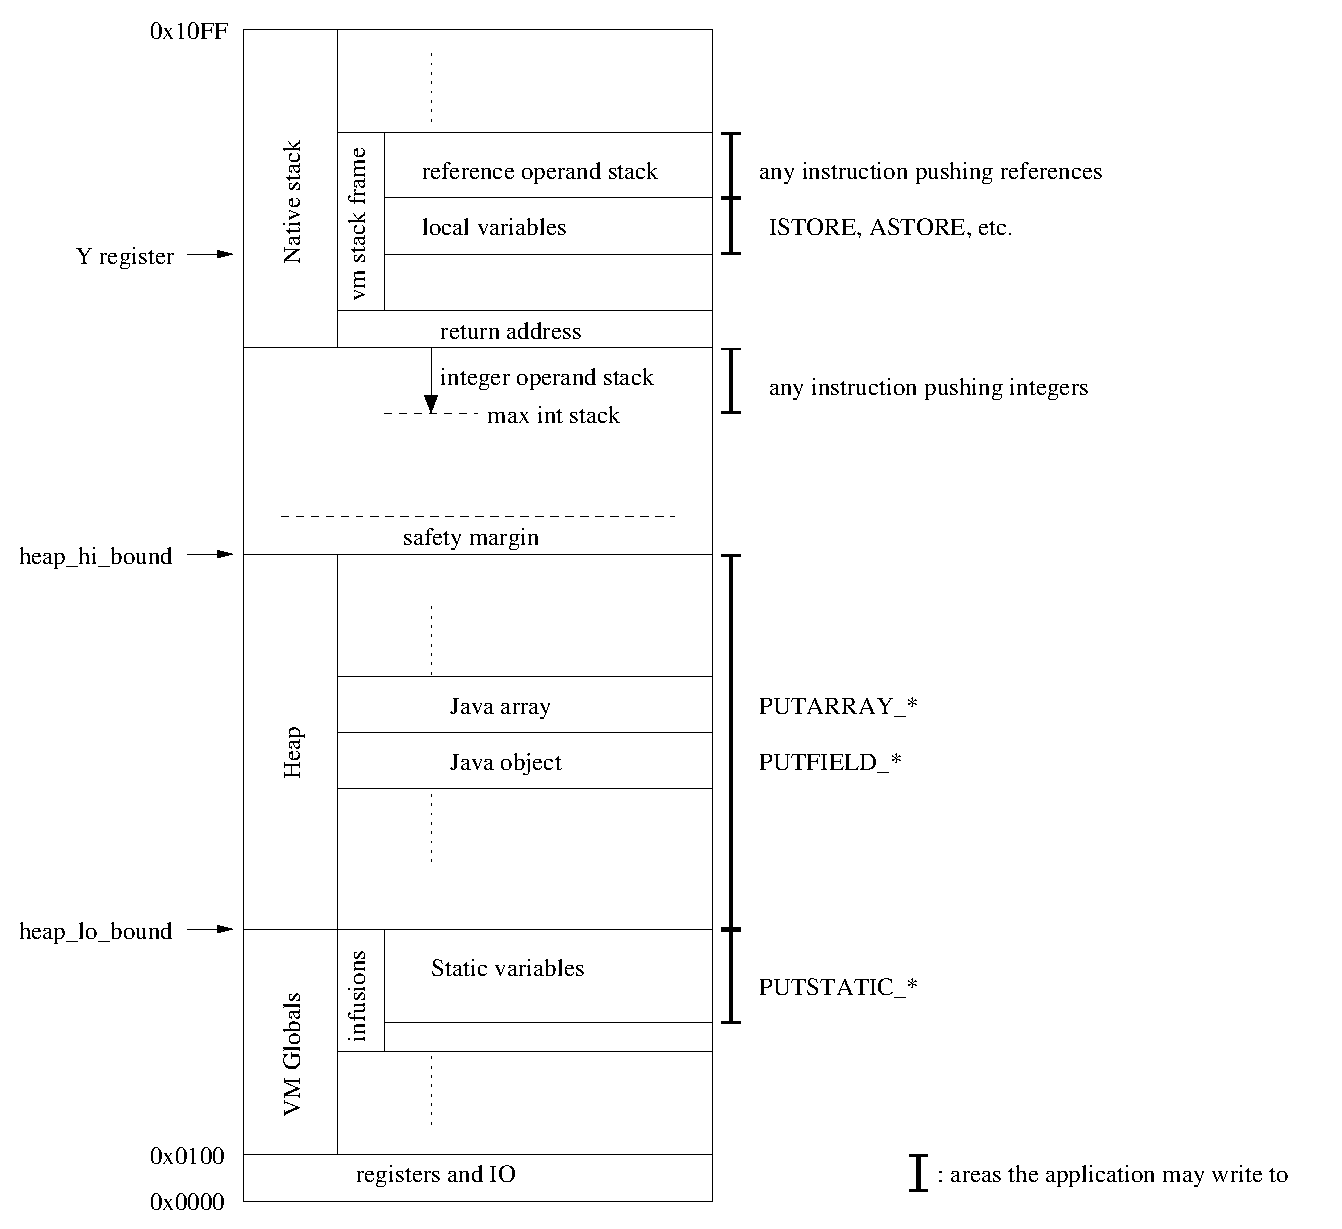
\includegraphics[width=\linewidth]{memlayout.eps}
\caption{Global memory layout and the areas accessible to the application}
\label{fig-memlayout}
\end{figure}

Figure \ref{fig-memlayout} shows the global layout of the VM's memory. At the bottom are the internal state of the VM, stored in a number of global variables, and a block with infusion descriptors which includes space for the static variables of each class in the infusion. This is followed by the application heap, which contains Java objects and arrays.

The native stack grows down in memory towards the heap. This contains a mix of native stack frames for internal VM functions, the application's VM stack frames, and the integer operand stacks which grow down directly on top of the native stack. The application's stack frames, shown in Figure \ref{fig-object-and-stack-frame-layout} consist of internal bookkeeping fields, space for local variables, and the reference operand stack.

Thus, the VM's private data and the application data are mixed in the node's memory. The application is only allowed to write to the areas indicated with bars to the right in Figure \ref{fig-memlayout}. Any write outside of these designated areas may corrupt the VM's internal state, and needs to be prevented by safety checks.

Having ensured control flow safety, we can rely on the fact that the VM will always execute complete bytecode instructions, and the application cannot skip past inserted run-time checks. Similar to control flow safety, we demonstrate memory safety by grouping instructions with respect to their memory writes, as shown in Table \ref{tbl-memory-write-instructions}, and defining the checks necessary for each category.

\begin{table}
\caption{Instructions writing to memory}
\label{tbl-memory-write-instructions}
    \begin{tabular}{ll} % NO SIMULATION DATA
    \toprule
    Type                                         & Writes to \\
    \midrule
    \midrule
    Any instruction pushing to the operand stack & The reference or integer stack \\
    \mycode{STORE}                               & A local variable in the current method's stack frame \\
    \mycode{PUTSTATIC}                           & A static variable in an infusion \\
    \mycode{NEW}                                 & The heap \\
    \mycode{PUTARRAY}                            & An array on the heap \\
    \mycode{PUTFIELD}                            & An object on the heap \\
    \bottomrule
    \end{tabular}
\end{table}


\subsection{The operand stack}
The VM will reserve space for the operand stacks based on the maximum stack depth in the method headers, so it needs to make sure the actual stack depth neither underflows, or exceeds the maximum announced in the header. Everything in this section applies equally to the integer and reference stack.

The VM creates a stack frame based on the method header, so at translation time it is known exactly how much space will be available at run time. Lightweight methods do not create their own stack frame, but depend on the caller's stack frame. Whenever an \mycode{INVOKELIGHT} instruction is translated, the VM needs to verify the stack frame of the current method has reserved enough free space for the lightweight method's stack (\ref{chk-sufficient-stack-space-at-invokelight}).

The effect of each instruction on the operand stack is known at translation time, so the stack depth can be verified in a single top to bottom pass. While translating a method, the VM maintains two counters indicating how many values are on the integer and reference stacks, and updates these counters for each instruction's stack effects. For normal methods both counters are initialised to 0, since they start with empty stacks. Lightweight methods start with their parameters on the stack, so for these the counters are initialised according to the number of arguments announced in the method header.

For each translated instruction, the VM checks there are enough values on the stack to consume its operands (\ref{chk-no-operandstack-underflow}), and that the maximum stack depth announced in the header is not exceeded after pushing its results (\ref{chk-no-operandstack-overflow}).

\paragraph{Branches}
The \mycode{BRTARGET} instruction poses a problem for this single pass approach since it can be reached from multiple locations, so the stack depth when entering this instruction is unknown.

The simplest solution is to require the stack to be empty at all branches. As mentioned in Section \ref{sec-optimisations-simple-stack-caching}, this is already the case for most code generated by \mycode{javac}.

Alternatively, the expected stack state at each branch target could be included in the method header, which would allow the VM to check the state matches this expected state at each branch and branch target. However, this is more complex and in practice the overhead for requiring an empty operand stack at branches is minimal: in our entire Java codebase only a few small modifications were necessary, which a future combined optimising infuser could do automatically.

Therefore, the VM only verifies the stack is empty at branches and branch targets (\ref{chk-stack-is-empty-at-branches}).

\paragraph{Invoke instructions}
Most bytecode instructions have a fixed effect on the stack, for example \mycode{IADD} will always consume two 32-bit ints and push another. We encode this in a simple table. Method calls require some more attention.

The \mycode{INVOKESTATIC}, \mycode{INVOKESPECIAL}, and \mycode{INVOKELIGHT} instructions all contain the id of the method that will be invoked. For these, the number of arguments and return type in the target method's header are used to determine the instruction's stack effects.
 
For \mycode{INVOKEVIRTUAL} and \mycode{INVOKEINTERFACE} the actual method that will be called depends on the object on the stack at run time. For these, the expected stack effect is determined based on the first implementation that matches the call. For valid code all implementations should have the same signature, and thus the same effect on the stack, but malicious code could send an implementation in a subclass that has different stack effects. Therefore, a run-time check (\ref{chk-invokevirtual-stack-effects-match}) is added that verifies the method called at run time has the same stack effects as the one used to verify the stack at translation time.

\paragraph{Return instructions}
Note that \mycode{RETURN} instructions do not need any special care. The stack depth in the method is verified using the instruction found in the bytecode. It is possible for a method to break the contract established in the method header, for example by using \mycode{RETURN} instead of \mycode{IRETURN} in a method that should return an int. However, this is still safe as long as the stack is empty after the return instruction, as checked by \ref{chk-stack-is-empty-after-return}.

Because the return value is passed back to the calling method in registers, the result of using an incorrect return instruction is that either the return value is discarded, or whatever happens to be in the registers is used as a return value. This may corrupt the application's own state, but not the VM's.

\subsection{\mycode{STORE}}
Local variables are accessed as an offset from the Y register, which is under control of the VM and points to the start of the local variables, as shown in Figure \ref{fig-memlayout}. Similar to the operand stack, the method header contains the number of variable slots that will be allocated in a normal method's stack frame. For lightweight methods, the VM checks \mycode{INVOKELIGHT} instructions to verify the caller has reserved enough local variable slots for the target method (\ref{chk-sufficient-locals-at-invokelight}), so the number of slots specified in a lightweight method's header is also guaranteed to be available at run time.

Local variables are written to using the \mycode{STORE} instructions. Each \mycode{STORE} instruction contains the index of the local variable slot to write to, so the VM only needs to check at translation time that the index of the local is within the range announced in the method header to guarantee it writes to a valid location (\ref{chk-local-variable-slot-exists}).

\subsection{\mycode{PUTSTATIC}}
Static variables are allocated globally before the application is started, based on number of static variables in the \emph{infusion} header. The \mycode{PUTSTATIC} instruction contains the id of an infusion, and the index of the target static variable slot. At translation time, the VM checks the referenced infusion exists (\ref{chk-static-variable-infusion-exists}), and the index is within the legal range (\ref{chk-static-variable-slot-exists}) for that infusion.

\subsection{\mycode{NEW}, \mycode{PUTFIELD} and \mycode{PUTARRAY}}
\label{sec-safety-heap-access}



%\begin{listing}
%   \centering
%   \begin{minted}{c-objdump}
%    heapcheck:                               cycles   bytes
%        lds  r0, heap_lo_bound               2        4
%        cp   ZL, r0                          1        2
%        lds  r0, heap_lo_bound + 1           2        4
%        cpc  ZH, r0                          1        2
%        brlo illegal_access_handler:         1        2
%        lds  r0, heap_hi_bound               2        4
%        cp   r0, ZL                          1        2
%        lds  r0, heap_hi_bound + 1           2        4
%        cpc  r0, ZH                          1        2
%        brlo illegal_access_handler:         1        2
%        ret                                  4        2
%   \end{minted}
%   \caption{Heap bounds check}
%   \label{lst-heap-bounds-check}
%\end{listing}

The final type of memory access is to the heap. The various \mycode{NEW} instructions used to create arrays and objects are fully implemented by a call to the VM, which only allocates new objects at a valid heap location and will terminate the application if it runs out of memory. Writes to object fields and array elements happen using the \mycode{PUTFIELD} and \mycode{PUTARRAY} instructions.

These instructions both work on an object reference, so a null reference bug could easily cause the VM to write to the lowest addresses. In the ATmega, the lowest 32 bytes of the address space are mapped to the CPU's general purpose registers, so this can cause very hard to diagnose bugs. Similarly, using a high out-of-bounds index into an array, malicious code could gain access to the native stack and, for instance, corrupt return addresses.

In some cases it may be possible to verify these operations at translation time, but this is hard without extensive analysis that would be too expensive for a sensor node. Therefore a run-time check is added when translating these instructions, which checks the target address is within the heap just before the actual write to memory (\ref{chk-memory-access-within-heap}).

\begin{listing}
    \centering
    \begin{minted}{c-objdump}
    heapcheck:
        lds  r0, heap_lo_bound
        cp   ZL, r0
        lds  r0, heap_lo_bound + 1
        cpc  ZH, r0
        brlo illegal_access_handler:
        lds  r0, heap_hi_bound
        cp   r0, ZL
        lds  r0, heap_hi_bound + 1
        cpc  r0, ZH
        brlo illegal_access_handler:
        ret
    \end{minted}
    \caption{Heap bounds check}
    \label{lst-heap-bounds-check}
\end{listing}

The VM stores the bounds of the heap in two variables: \mycode{heap_lo_bound} and \mycode{heap_hi_bound} as shown in Figure \ref{fig-memlayout}. Each heap access instruction calculates the address to write to in the ATmega's Z register. Just before the write to the heap, the VM inserts a \mycode{CALL} to the \mycode{heapcheck} function shown in Listing \ref{lst-heap-bounds-check}. This function checks the address in Z is within these bounds. If not, it jumps to the \mycode{illegal_access_handler}, allowing the VM to terminate the application. This adds 22 cycles overhead for each array or object write, and 4 bytes code size overhead for the \mycode{CALL} instruction.

The actual write to the heap is often done by an offset from Z using the ATmega's \mycode{STD}, or 'store indirect with displacement' instruction, that allows writes to a fixed offset of at most 63 bytes from Z. For example, to write to object fields who's offset within the object is known at translation time, the VM simply loads the object's address into Z and uses \mycode{STD} to write to the correct offset.

This means the write could target an address at most 63 bytes above the end of the heap. One way to prevent this is to avoid the \mycode{STD} instruction, and instead use the \mycode{ADIW} instruction to first add the offset to Z and then use the normal \mycode{ST} instruction to store without displacement. However, this would add an overhead of 2 bytes and 2 cycles. Instead we reuse the same small safety margin mentioned in Section \ref{sec-control-flow-safety-return-instructions} for check \ref{chk-no-nativestack-overflow}. Reusing the same margin for both cases is safe because the VM can never write to a heap object and execute a function in the VM or \mycode{libc} at the same time.

\paragraph{Alternatives}
We considered several alternative implementations for \mycode{heapcheck}. Since the \mycode{CALL} and \mycode{RET} instructions are expensive, 7 cycles can be saved by inlining the check instead of calling it. However, this increases the code size overhead from 4 bytes to over 30 bytes, which we consider too high.

If the top and bottom boundaries of the heap are aligned at 256 bytes, this eliminates the need to check the lower byte of the Z register. This saves 6 of the 22 cycles, but wastes RAM since some bytes below and above the heap would have to remain unused. Since RAM is such a scarce resource and the performance gain is limited, we decided against this.

Finally, 8 cycles can be saved by keeping the bounds in registers instead of memory, which removes the need for the \mycode{LDS} instructions. However this reduces the performance of the stack cache since these registers would not be available for stack caching. Which of these affects performance more depends on the code being executed. We evaluate the difference in Section \ref{sec-evaluation-run-time-cost}. Since having the bounds in registers is more complex to implement, thus increasing VM size, we choose to keep the bounds in memory.

\paragraph{Heap corruption}
Since the garbage collector compacts the heap when it frees any memory, the heap is always split into an in-use part and a free part. A pointer in the VM points to the first free byte. This pointer is moved forward when memory is allocated, and moved backward when the garbage collector compacts the heap.

The in-use part of the heap is made up of chunks, which have a small header indicating their size. The heap access check only verifies a write is to an address within the heap, but not that the address is a correct address within the target object. Code may still corrupt parts of the heap, including these heap headers.

This does not break the safety guarantees since these heap headers are not used until control is returned to the VM. The headers are only used by the garbage collector, so before the garbage collector starts, the VM checks the intergrity of the heap headers (\ref{chk-gc-heap-integrity}), which must form a consistent chain of chunks, ending at the first free byte.



\section{Comparison to other systems}

\begin{table}
\caption{Comparison of CapeVM's safety guarantees to source code approaches}
\label{tbl-safety-comparison-source-code-approaches}
    \begin{tabular}{p{.35\textwidth}p{.28\textwidth}p{.27\textwidth}} % NO SIMULATION DATA
    \toprule
                                                & CapeVM and                                  & Source code approaches \\
                                                & native code approaches                      & \\
    \midrule
    \midrule
    Safety checks added/verified at             & The node                                    & The host \\
    Protects                                    & The VM                                      & The VM and the application \\
    Protects against malicious code             & Yes                                         & No \\
    Detects certain programming errors          & No, but could be added                      & Yes \\
                                                & ~~~ at a cost                               & \\
    \bottomrule
    \end{tabular}
\end{table}

This section compares CapeVM's approach to other systems providing safety. Section 4.10 of the Java Virtual Machine Specification \cite{Lindholm:2017vu} specifies a number of checks an implementation must do to comply with the standard. CapeVM's checks are different in two ways: First, they are defined at a lower level, specific to our VM's implementation. Second, since CapeVM's goal is only to ensure the application cannot corrupt the VM, its checks are less restrictive than the JVM specification.

For example, CapeVM allows out of bounds array indexes. While incorrect, these do not violate the safety guarantees as long as the write stays within the heap. Out of bounds array access indicates a bug in the programme, and failing early instead of corrupting the application's state usually makes it much easier to find the bug. CapeVM's checks ensure malicious code cannot corrupt the VM, but they do not prevent such programming errors from corrupting the application's own state, unless they also violate the safety constraints.

Section \ref{sec-state-of-the-art-source-code-safety} introduced a number of systems such as Safe TinyOS \cite{Cooprider:2007ub} that work on the source code level. While seemingly similar, they are actually the reverse in the sense that their more fine-grained checks do prevent certain programming errors from corrupting the application's state, but since the node assumes the necessary checks to be in place, they cannot guard against malicious code sent to the device. Because in these systems the safety checks are added by the host, more complex analysis can be done on the source code to prove certain operations to be safe at compile time, which reduces the number of necessary safety checks and thus the run-time overhead.

The checks in the JVM's specification both protect the VM against malicious code and the application from certain programming errors. Desktop JVMs, like the host in Safe TinyOS, have ample resources to do the analysis necessary to reduce the overhead of fine-grained checks. On a sensor node we argue the two goals require two separate solutions.

While CapeVM's checks could be extended to provide the same level of safety as Safe TinyOS, to do so would require extending the existing checks to include the size of the object or array that is being accessed, which would make them considerably more expensive. Since CapeVM adds the safety checks on the node, it lacks the resources necessary to do the analysis that allows Safe TinyOS to eliminate many checks. Instead, CapeVM must conservatively check each access.

If the goal is to protect the application from programming errors that could corrupt its own state, this implies control over the code, and an approach similar to that of Safe TinyOS will be more efficient. Safe TinyOS works on native nesC code, but a similar system could be developed for Java where the checks inserted by the host are implemented as new bytecode instructions to mark array or object accesses than need run-time checking.

The difference between both approaches is summarised in Table \ref{tbl-safety-comparison-source-code-approaches}. For some applications both may be useful. For example, in a system like the Amulet smart watch, CapeVM's safety checks are useful to isolate an untrusted application from the VM. At the same time, more fine-grained checks may be added to detect buggy applications. Since these checks are for the application's benefit only, the node does not need to be able to verify them and adding these checks on the host, similar to Safe TinyOS, will lead to less overhead compared to extending the checks added by the node.




\subsection{SensorScheme}
Next, we will compare the approach taken by CapeVM to three existing systems that provide safety on the node. First, SensorScheme is the only sensor node VM to explicitly mention safety, although it does not describe many the details.

SensorScheme is a LISP dialect, so both code and data are stored as lists. In SensorScheme memory is organised as a collection of fixed-sized \emph{cells} that make up these lists. Since the cells are managed by the VM this inherently gives it a level of safety, and run-time checks are added to check the datatypes and length for each operation. Since it is an interpreter, it has a large run-time overhead, which makes the added overhead of these checks insignificant.




\subsection{\emph{t-kernel}}
In addition to safety, \emph{t-kernel} \cite{Gu:2005un, Gu:2006ww} also provides a form of virtual memory which makes it hard to compare to CapeVM directly. The authors name OS control and memory integrity as the two primitives the system needs to provide in order to protect the kernel from the application.

\paragraph{OS control and control flow safety}
OS control is defined as the ability of the OS to take control of the CPU. The authors note that

\begin{displayquote}“Traditionally, the CPU control is guaranteed by privilege support and clock interrupts. However, many microcontrollers used by sensor nodes do not have privilege support. The application can disable interrupts and occupy the CPU for an arbitrarily long time.”\end{displayquote}

To implement its virtual memory features and safety guarantees, \emph{t-kernel} extensively rewrites, or \emph{naturalizes}, the application's binary code at run time, on demand, one 256-byte page at a time. As a result, addresses in the original binary do not match the physical addresses in the naturalized pages. This is solved by replacing all branching instructions, including calls, returns, etc, with calls back to the kernel, which then looks up the corresponding physical address.

This causes a slowdown of up to 30x. To reduce this overhead, these calls back to the kernel are replaced with a direct jump after the first transition occurs for forward branches. Backward branches are replaced with code that first increment an 8-bit counter, and calls back to the kernel when this reaches zero. This guarantees the kernel gets back control at least once for every 256 backward branches, without depending on a timer, but at the cost of a slight overhead. Control flow safety is not explicitly discussed, but is guaranteed by the same mechanism. Since each branch targets a virtual address, which is translated to a physical address by the kernel, the kernel can ensure the physical address is correct.

Compared to \emph{t-kernel}, it is easier for CapeVM to guarantee it can regain control of the CPU. Since the VM offers no functions for the application to turn of interrupts or modify timers, it \emph{can} simply use an interrupt to ensure it periodically regains control of the CPU.

% TODO: mention that this is rather weak since t-kernel could just forbid disabling interrupts (it's a simple instruction to check for). Also it doesn't discuss the possibility for malicious code to brick the device by putting it in deep sleep mode without any timers to wake it up. (can you do that?)

\paragraph{Memory safety}
Memory in \emph{t-kernel} is split into three regions: (i) physical addresses that map to IO ports, special registers, etc, (ii) the stack, and (iii) the heap. Most accesses, to local variables, parameters, register saves and restores, etc are to the stack. The naturalization process ensures stack access is safe, although the paper does not go into details. Stack access is optimised, but there is some overhead for certain types of access. In the worst case, indirect addressing with displacement, this takes 5 instead of 2 cycles. In CapeVM, local variable access incurs no extra overhead from safety checks, since it can determine at translation time whether or not it targets a valid local variable slot.

\emph{t-kernel}'s virtual memory provides the application with a 60 KB heap. This is divided in 16 byte pages, some of which are kept in buffers in RAM. Each buffered page has a header indicating its virtual memory starting address. When the application accesses the heap, \emph{t-kernel} searches the pages in RAM, starting with the one used for the most recent access. If the required page is not in RAM, it is swapped in from flash. Besides providing virtual memory, this also guarantees safety since a heap write always writes to a buffered page, and the entire virtual heap is assigned to the application.

Access to the heap is both considerably slower than stack access, and highly variable. The paper lists a benchmark which does repeated heap accesses without swapping. This takes 16 cycles, compared to 2 for a normal memory access. The paper does not mention whether the benchmarks targets different pages, but the low overhead would suggest it may target the same address for every write, which means the first page the kernel examines is the correct one. If the required page is not found in RAM, it is swapped in from flash, which takes over 180,000 cycles.

The best case access of 16 cycles is comparable to CapeVM's 22 cycle overhead for heap access, but will rise if multiple pages need to be searched by the kernel, or if pages need to be swapped in from flash. Unfortunately the paper does not mention how many pages are buffered in RAM, but it is clear applications with more data - the ones that would benefit from having a larger virtual memory - will incur a higher overhead, either from having to scan more buffered pages, or from having to do more swapping.

In conclusion, \emph{t-kernel}'s performance overhead should be slightly higher than CapeVM's in most cases. In addition, the extensive rewriting of the binary code adds a large code size overhead, reported at a 6-8.5x increase.




\subsection{Harbor}
Harbor guarantees safety by adding checks on the host. A verifier on the node then verifies all checks are in place before executing the programme. While checks are added by the host with its ample resources, Harbor is still bound by the limited resources on the node since the node needs to be able to verify correctness.

\paragraph{Control flow safety}
In a Harbor application, run-time checks are added to protect writes. To guarantee applications cannot jump past these run-time checks, Harbor disallows computed branches so the verifier can check the target address of each branch.

Function returns could also be used to jump to an arbitrary location if the return address can be corrupted. To prevent this, Harbor uses function entry and exit stubs that store the return address in a 'safe stack' in a reserved section of memory not accessible to the application. This adds an overhead of 76 cycles per function call.

\paragraph{Memory safety}
Memory safety in Harbor differs significantly from CapeVM. The entire address space is split into fixed sized blocks, each of which can be assigned to a module. A memory map keeps track of the ownership of each block.

Harbor supports multiple modules, and both the block size and the maximum number of modules are parameters that can be changed. The overhead for storing the memory map is 256 bytes for an 8-byte block size and maximum of 8 modules, which are the defaults used in the paper. Using only 2 modules, which is sufficient to isolate the OS from the application, this is reduced to 128 bytes. Increasing the block size will also reduce the size of the memory map, but at the cost of greater fragmentation.

All memory writes are preceded by a call to the \mycode{write_access_check} function, which checks the current module has permission to write to the target address. This imposes a run-time overhead of 65 cycles per write.

CapeVM only needs a run-time check for writes to the heap, while Harbor checks \emph{all} writes, including local variables. This, combined with Harbor's more expensive \mycode{write_access_check} function, suggests its overhead will be significantly larger than CapeVM's.

\paragraph{Verifier}
Although Harbor's safety checks are added on the host, the correctness of the system only depends on the verifier running on the node. This verifier is a relatively small and simple component.

This is a significant advantage of Harbor's approach. Malicious attacks often exploit bugs in the system they are trying to corrupt. Compared to more complex systems like \emph{t-kernel} and CapeVM, the simplicity and small size of Harbor's verifier reduces the chance of exploitable bugs, but this comes at the cost of an increased run-time overhead.

